\documentclass{article}
\usepackage{graphicx}
\usepackage[]{mcode}

\title{Mandatory 1}
\author{INF4300 \\ Autumn 2015}

\begin{document}
\maketitle{}
\break
\section{Analyzing the textures}

Here i will describe what characterizes each texture, and how they differ.  
\subsection{Mosaic 1}
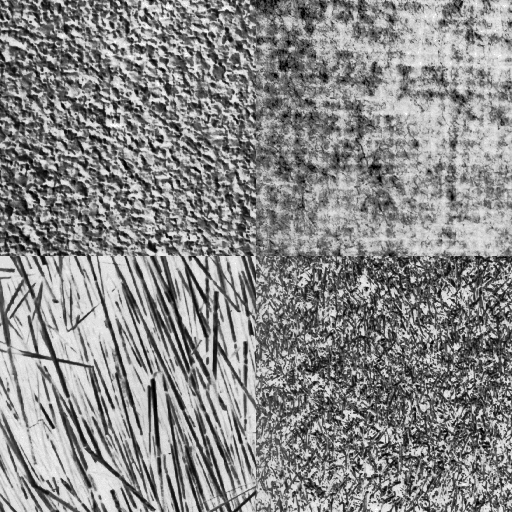
\includegraphics[totalheight=12cm]{mosaic1.png}
\subsection{Texture 1(top left)}
The texture can look a bit like mountains with shadows seen from above.
Texture have a weak direction diagonaly down, it can look line the texture have a frequency at around 20 if we go diagonaly upwards, if it is any frequensy at all. It is much black pixels and some white, so the variance is medium. The homogenity are also medium.
\subsection{Texture 2(top right)}
The texture have a weak square formation. It have much black areas on to the left, and more white to the right of the picture. The texture direction is squared. The frequency are 42 vertival and horisontal. Variace and homogenity are low. The texture elements are around 12x12 on this picture.   
\subsection{Texture 3(botom left)}
The texture look like black straws. Going in a 60degree angle down. The frequency is vary much, but it is often around 9 pixels between the straws. Variance and homogenity are very high. The straw elements are around five pixels wide. 
\subsection{Texture 4(buttom rigth)}
The texture have some vertical and some diagonaly lines, but not very significant. It also have many random white areas that vary in sizes from 5x5 to 20x20. It is hard to spesify a distict frequency, but it can look like vertical lines. The varance are medium, and homogenity is high.
\subsection{Mosaic 2}
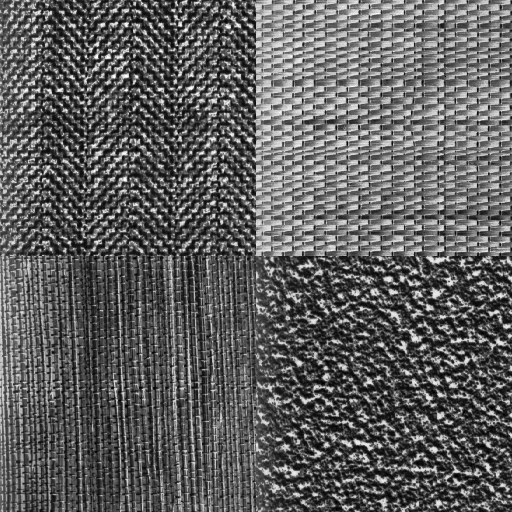
\includegraphics[totalheight=12cm]{mosaic2.png}
\subsection{Texture 5(top left)}
This picture have a very distinct pattert. The pattern look like stairs going up and down when you traverse the picture horisontaly. The the horisontal frequency are 3, and frequency vertical are 20. 
Variance and homogenity are medium. 
\subsection{Texture 6(top right)}
This pattern have a two very distict textures.The first texture have retangular elements in horisontal direction, combined with horisontal lines and smaller horisontal rectangular elements. In some places in the picture, the pattern breaks. Horisontal frequansy are 12, and vertical are 40. The other pattern is a wave formed pattern in a 30 degree angle. It look line it lays on top of the retangular elements, so the frequency is the same as the square vertical frequency. Variance and homogenity are low. Most of the elements have a size on 42x12
\subsection{Texture 7(botom left)}
The picture look like, and I am quite sure it is straw wallpaper. Horisontal frequency are 40. Texture direction are vertial , variance and homogenity are medium.
\subsection{Texture 8(buttom rigth)}
This pattern look much like top left on mosaic1. It look like mouintais or desert seen from above. It have no spesific direction or frequency. It have som clear white small elements that vary in size. It have a bit high homogenity and variance because it have black and white areas. 

\section{Visualizing GLCM matrices}
\subsection{Subimages}
Starting with creating subimage for all texture, calling them texture[1-8] in matlab. 
\subsection{Histogram}
After looking at histograms for all the subpictures, i choose to histogramtransform them, so it will easier to work with them later on.\\
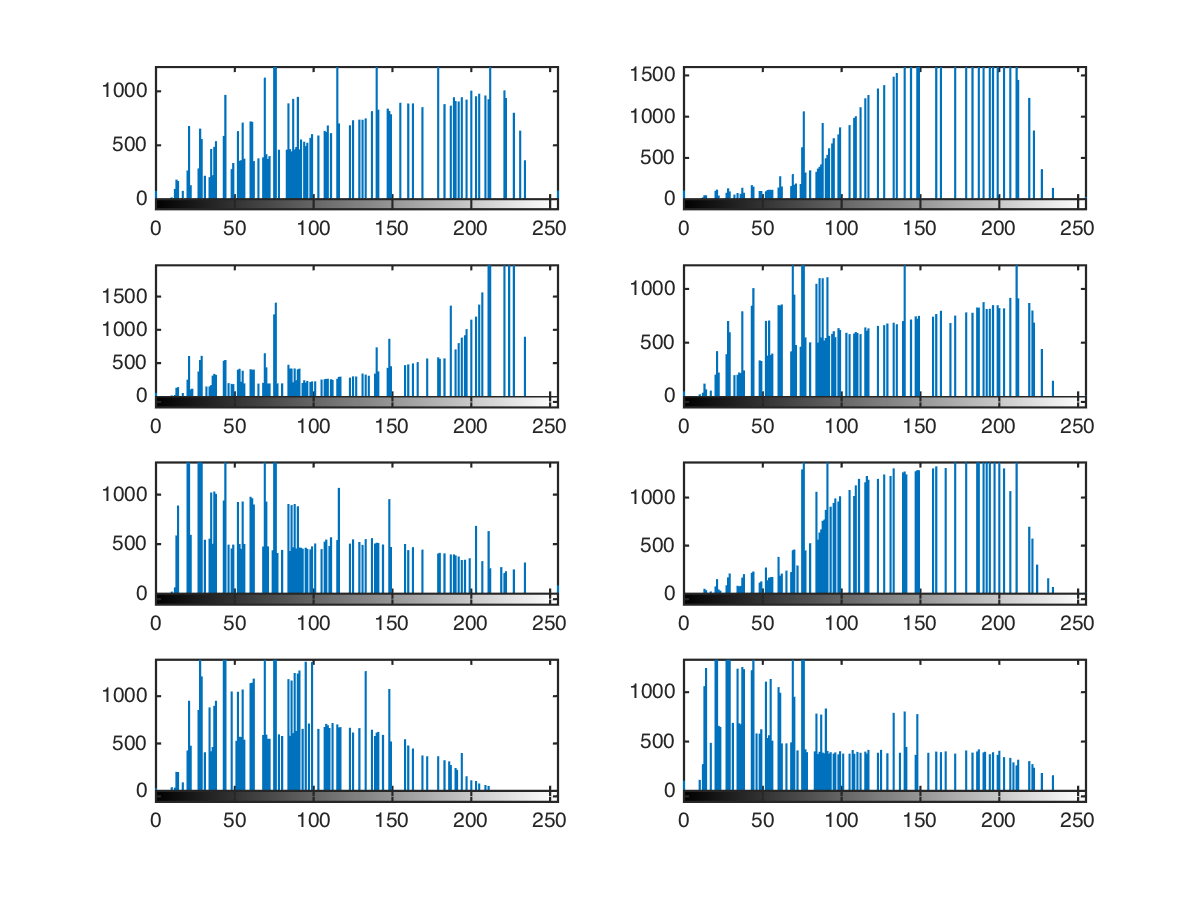
\includegraphics[totalheight=8cm]{detailhist.png}
    	
\subsection{GLCM paramaters}    	

I will try to find parameters that i will use til capture the tecture in the picture. I will use $dx$ and $dy$ where $dx$ are movement in vertical direction, and $dy$ are in horisontal direction. Example: $dx = 10, dy = 0$ will be de same ac $\theta = 0, d = 0$, that mens 10 vertial and 0 horisontal.  
I will use directional GLCM in all textures. \\
\begin{itemize}
\item[\textbf{Texture 1}] I this texture i will try to folow the "hills" formation. I will use $(3, 4)$ and $(2, 2)$  to capture the hill texture. \\
\includegraphics[totalheight=5cm]{t1plot.png}

\item[\textbf{Texture 2}]
Here i will try to folow the squares, that go in horizontal and vertial direction with a weak angle. It is very week. I will use $(10, -1)$ and $(-1, 10)$\\
\includegraphics[totalheight=5cm]{t2plot.png}

\item[\textbf{Texture 3}]
Here i will forlow the "straws". Since most of them go in the same direction i will follow them. $(10,3)$ parameter will hit the straws in most cases. \\
\includegraphics[totalheight=5cm]{t3plot.png}

\item[\textbf{Texture 4}]

Here i will use $(10, 0)$ and $(0, 10)$ that hopefully will be a big variance since it hit no texture elemets. 
\\
\includegraphics[totalheight=5cm]{t4plot.png}

\item[\textbf{Texture 5}]
Naturally I will try to hit the stair formation in this texture. I will use $(6, 6)$ and $(6, -6)$. They will follow the stair formation. 
\\
\includegraphics[totalheight=5cm]{t5plot.png}

\item[\textbf{Texture 6}]
Here i will follow the squares, and try to hit the same intensity on each pixel to get a low variance. I will use $(10, 20)$, and $(0, 10)$\\
\includegraphics[totalheight=5cm]{t6plot.png}

\item[\textbf{Texture 7}]
Here i will follow the vertial diretion in the texture. $(10, 1)$
\\
\includegraphics[totalheight=5cm]{t7plot.png}
\\ We can se the texturelines in the GLCM picture.

\item[\textbf{Texture 8}]
$(4,4)$ Here and try to get low variance when folowing the pattern.
\\
\includegraphics[totalheight=5cm]{t8plot.png}\\
The resultpicture got low variance. 
\\
\end{itemize}

\section{GLCM feature images}
In this section i did not find out how to compute the GLCM cluster shade. I will show the glcm energy insted. Parameters will be the same that i used in part a. 
\subsection{Texture 1}
Here i am chooseing a 11x11 window, because so I can see a full texture element. \\
\includegraphics[trim=75 140 0 140,clip,totalheight=5cm]{tw1plot.png}

\subsection{Texture 2}
On this texture i will use a 31x31 window, so i can get  a full square texture element. 
It is not posible to see the formation square formation on the window because it is to weak.\\
\includegraphics[trim=75 140 0 140,clip,totalheight=5cm]{tw2plot.png}
\subsection{Texture 3}
I use a 51x51 in this texture, so I can se some straws. \\
\includegraphics[trim=75 140 0 140,clip,totalheight=5cm]{tw3plot.png}
\subsection{Texture 4}
A 16x16 on this picture will be sufficent. \\
\includegraphics[trim=75 140 0 140,clip,totalheight=5cm]{tw4plot.png}
\subsection{Texture 5}
When i make a 41x41on this texture, it is easy to see the stairs. \\
\includegraphics[trim=75 140 0 140,clip,totalheight=5cm]{tw5plot.png}
\subsection{Texture 6}
31x31, are good on this one, so I can get a whole texture element.\\ 
\includegraphics[trim=75 140 0 140,clip,totalheight=5cm]{tw6plot.png}
\subsection{Texture 7}
A 21x21 window, will show the texture here. \\
\includegraphics[trim=75 140 0 140,clip,totalheight=5cm]{tw7plot.png}
\subsection{Texture 8}
This texture is small. A 16x16 window is big enough here. \\
\includegraphics[trim=75 140 0 140,clip,totalheight=5cm]{tw8plot.png}

\section{Segment the GLCM feature}
\subsection{Mosaic 1}
In this section i will take all the parameters i used on the textures in section A to make a GLCM for mosaic 1. The first result is quite messy. I decite to use a 50x50 median filter to clear thing up. 
\\
\includegraphics[totalheight=8cm]{img1plot.png}\\
This is the result after the 50x50 filter:
\\
\includegraphics[totalheight=8cm]{img1eplot.png}
\\
Then I am treshholding to get the final result, se the threshold values in the plot. I used two  stats pictures on in most cases to get a better result.\\
\includegraphics[totalheight=10cm]{img1tplot.png}
\subsection{Mosaic 2}
Here i will do the same that i did with mosaic 1. I still use the same parameters.
\\
\includegraphics[totalheight=8cm]{img2plot.png}\\
This is the result after the 50x50 filter:
\\
\includegraphics[totalheight=8cm]{img2eplot.png}
\\
Not i am treshholding to get the final result:\\
\includegraphics[totalheight=10cm]{img2tplot.png}
After segmentet this picture, i found out that my GLCM parameters could be better. 


\end{document}